\cleardoublepage

\chapter{Conclusión y mejoras}
\label{ch:Capitulo6}


El estudio requerido para la creación de una suite domótica ha representado un reto dada la extensión de opciones tecnológicas, estándares establecidos y protocolo de arquitectura y comunicación disponibles. Aun no habiendo podido experimentar con pruebas reales todos los estudios planteados en el estado del arte, puede confirmarse una selección adecuada de tecnologías para abordar un proyecto de \gls{iot} que enfrente los problemas característicos de una suite domótica.

\vspace{1cm}

El uso del protocolo \gls{mqtt} ha demostrado ser una de las opciones más sencillas para abordar la comunicación y transferencia de mensajes entre nodos y \gls{gateway}. Posee una baja carga de consumo energético en las placas microcontroladoras y facilita la gestión de identidades de dichas placas en la red domótica gracias al planteamiento de publicación y subscripción de topics. Además, debido al uso de cadenas de caracteres en formato \gls{json}, es sencillo manejar las respuestas y peticiones del servidor de la aplicación. Las primeras pruebas realizadas sobre el protocolo \gls{http} demostraron un mayor consumo energético y de proceso como resultado de ejecutar un servidor web en cada placa individualmente. Esto implicaba que las respuestas por parte de las placas pudieran demorarse hasta 5 segundos cuando el servidor solicitaba información a las mismas. Estas placas además, estuvieron conectadas a pequeñas baterías de 5v con capacidad para 3500mA y fueron agotadas en menos de 4 horas. En las pruebas sucesivas, el código de las placas utilizo el protocolo \gls{mqtt} reduciendo los tiempos de respuesta de las placas a las peticiones del servidora un máximo de 2 segundos y la dirección de las mismas baterías se amplio hasta 8 horas. Ambos protocolos están basados en el estándar \gls{tcp} y eso permite una comunicación más confiable entre dispositivos, permitiendo incluso plantear el uso de técnicas de cifrado para la comunicación.

\vspace{1cm}

El uso de la tecnología \gls{wifi} es un acercamiento válido en un hogar de pocas habitaciones, pero la atenuación de señal es evidente en las paredes de las habitaciones, y si el \gls{gateway} se encuentra ubicado a una distancia superior a tres habitaciones de un nodo, la señal se ve lo suficientemente debilitada para que se produzcan pérdidas de paquetes o caídas de la conexión. Esta restricción debe ser tenida en cuenta en despliegues, ya que la estructura de los hogares es muy variable, y cada elemento arquitectónico del edificio posee un impacto diferente en la atenuación de las señales, por ejemplo, un muro de carga posee un mayor grosor que un muro divisorio, y la degradación de la señal es más notable en el primero. Igualmente, los suelos que separan los pisos son aún más restrictivos que los propios muros, en los pisos dúplex o chalet de varias plantas, si la señal tiene su origen en una habitación en el extremo opuesto de la habitación a la que queremos llegar, estando ésta además en una planta distinta, generalmente es poco probable que la señal llegue con suficiente calidad como para operar con normalidad. Otras tecnologías inalámbricas como \gls{6lowpan} podrían resolver estos casos con mejor desempeño, ya que poseen un mayor alcance. También puede valorarse explotar capacidades adicionales del chip \verb|ESP8266| integrado en las placas utilizadas en este prototipo para realizar un despliegue en malla, que permitiría a los nodos actuar como enrutadores de otros nodos, ampliando así el alcance total de la red en la distribución del hogar. Esta opción, sin embargo, debe ser sopesada en función del coste energético que implica en los nodos.

\vspace{1cm}

Sobre la cuestión de consumo energético de los nodos y el propio \gls{gateway}, es evidente que un nodo cuya duración de batería es inferior a medio día, no es práctico ni siquiera como prototipo. Hay que considerar en base a las medidas tomadas mediante un polímetro, que el uso normal de \gls{wifi} en los nodos de este proyecto consumen entre 50mA a 150mA, esto manteniendo una conexión constante en la red. Las placas microcontroladoras que en su \gls{soc} instalan el chip \verb|ESP8266|, disponen de funciones de hibernación que permiten apagar la mayoría de los elementos del nodo reduciendo de manera notable dicho consumo. Una estrategia valida en un despliegue de \gls{iot} puede aprovechar esta capacidad reduciendo el numero de comunicaciones entre el nodo y el \gls{gateway}, haciendo que la aplicación del servidor requiera de tomas de medidas programadas cada cierto tiempo en vez de manera constante o bajo demanda del usuario. en todo caso, este problema responde a si la alimentación de las placas es suministrada por baterías o se encuentran conectadas a la red eléctrica del hogar. Sólo en el primer caso las cuestiones de consumo son realmente relevantes.

\vspace{1cm}

A continuación se describen en distintas secciones como abordar los problemas mencionados a partir del desarrollo ya realizado en el prototipo, y mejoras de diseño e implementación que han quedado fuera del alcance original del proyecto.

\section{Refuerzos de la seguridad en la comunicación inalámbrica}
\label{ch:Capitulo6.1}
La librería pubSubClient~\cite{pubsubclientapi} utilizada en la generación de \gls{sketch} esta implementada para ser simple de usar. Sin embargo, tiene limitaciones en lo que respecta al cifrado de conexiones cliente-servidor mediante el protocolo \gls{mqtt}. No posee soporte para conexiones cifradas \verb|SSL/TLS|. Existen librerías ya disponibles de este protocolo que pueden aportar estas funciones, o ampliar la utilizada en este proyecto apoyándose en otras librerías que complementan la seguridad de las conexiones. Una aproximación deseable en el proyecto consta de reforzar dos puntos concretos de las conexiones inalámbricas de la suite domótica. Primero, establecer conexiones con la red \gls{wifi} mediante librerías mas robustas como \verb|WiFiClientSecure| que admite \href{https://arduino-esp8266.readthedocs.io/en/latest/esp8266wifi/client-secure-class.html}{cifrados asimétricos} con firma y verificación. 

\vspace{1cm}

El segundo paso requiere que el \gls{broker} de información del nodo principal resuelva las conexiones mediante el protocolo \gls{tls} en lugar de \gls{tcp} simple. Esta estrategia debe estudiarse antes de su implementación, ya que este protocolo, siendo más seguro, implica una mayor sobrecarga en la red con los \gls{handshake} de conexiones de corta duración, como ocurre con los actuadores, cuya comunicación se limita a recibir un comando y reportar un resultado. También debe considerarse la mayor carga de proceso que se aplica a los dispositivos y el propio nodo principal. En una red con una veintena de dispositivos que establecen comunicaciones de corta duración con contenidos de mensajes de apenas un par de decenas de caracteres, la sobrecarga de comunicación puede ser detrimental hasta el punto de hacer que la suite funcione anormalmente lenta. Por ello, la primera capa de cifrado en la red inalámbrica será una ampliación obligatoria y la segunda capa debe ser estudiada antes de su aplicación.

\section{Mejora en la cobertura inalámbrica de la suite domótica}
\label{ch:Capitulo6.2}

En términos de conectividad inalámbrica, la distancia de despliegue física de dispositivos está limitada al rango de emisión del adaptador \gls{wifi} que actúa como router. En este proyecto, el nodo principal de la suite domótica es dicho proveedor de red y los dispositivos se conectan dentro de su rango operativo. Las atenuaciones de señal son particularmente notables dentro de una casa, ya que existen múltiples elementos arquitectónicos como paredes, suelos y columnas, así como la presencia de otros dispositivos con funciones de conectividad inalámbrica. De hecho, una suite domótica, en carácter general siempre va a contar con estas dificultades como norma. Por ello debe plantearse una estrategia que establezca una zona de conexión con una señal estable y de un alcance a diez metros, a partir del cual se hace notable la caída de las señales \gls{wifi} emitidas por un punto de acceso, tal y como se recoge en un articulo de la universidad de Stanford sobre modelado de atenuaciones de señales \gls{wifi}, apartado 3, "Modeling Attenuation Indoors"~\cite{faria2005modeling}.

\vspace{1cm}

Aunque existen repetidores de señales que pueden ampliar el rango efectivo de una \gls{wlan}, en realidad, se están generando nuevos puntos de acceso con nombres distintos, y esto complica mucho el despliegue de nuevos dispositivos en la red de la suite domótica, teniendo que preveer qué nombre de \gls{wlan} le corresponde a un dispositivo que, por no estar a un alcance óptimo del nodo principal, debe conectarse a un repetidor concreto que le suministre mejor red. Incluso si se resuelve este problema, solo estaríamos consumiendo más tomas de corriente para alimentar dichos repetidores. Pero los chips \verb|esp8266| utilizados en este proyecto disponen de la capacidad de ser desplegados con una configuración de \gls{wifi} en malla. Conocido como \gls{wifi} Mesh, se trata de una arquitectura de comunicación inalámbrica donde cada dispositivo actúa como enrutador en la red, siendo cada uno un punto de acceso para otros nodos, lo que permite desplegar dispositivos mas allá del alcance del router del nodo principal.

\section{Actualización de código OTA en dispositivos}
\label{ch:Capitulo6.3}
El despliegue de nuevos dispositivos en la red domótica mediante una primera conexión \gls{usb}, ha demostrado evitar errores característicos de sincronización inalámbrica como ocurre en dispositivos de las marcas comerciales estudiadas en el estado del arte. Esto se debe principalmente a que no es necesario una etapa de sincronización y verificación por parte del usuario, ya que al conectar una placa al \gls{gateway}, se cargan todos los credenciales necesarios para las sucesivas conexiones. Sin embargo, existen ciertos escenarios donde poder alterar el código de las placas sin necesidad de volver a conectarlas al \gls{gateway} con una conexión alámbrica se puede convertir en un requisito primario. A tal fin, las placas que integran módulos \verb|ESP8266| disponen en sus librerías de capacidad de subir nuevo código mediante conexión \gls{wifi}. Esto es un gran avance respecto a las placas de Arduino originales que requerían de la ampliación física de hardware mediante los denominados \verb|shields| los cuales incluso no ofrecían esta capacidad en sus productos comerciales iniciales e implicaban la creación de nuevos dispositivos de hardware que solucionaban esta problemática. Puede observarse un ejemplo de implementación de esta idea en un trabajo de tesis realizado en la UPC nombrado "Design of an Arduino shield for ota programming"~cite{campa2013design}.

\vspace{1cm}

Un escenario previsto que podría beneficiarse son los cambios en la configuración \gls{wifi} del \gls{gateway}. Si al verse comprometida la contraseña de acceso inalámbrica a la red domótica, el usuario quisiera cambiar este parámetro, esto implicaría conectar todas y cada una de las placas ya desplegadas mediante \gls{usb} al \gls{gateway} para subir la nueva contraseña al código. Sin embargo, con la estrategia inalámbrica, podría ejecutarse un procedimiento que aplicase este cambio en todas las placas. Esta misma estrategia es aplicable a la hora de mejorar el código de las placas mediante refactorizaciones o actualizaciones de las librerías, lo cual permite mantener un sistema domótico actualizado y más fácil de mantener.

\section{Ampliando el nodo principal con interfaz táctil}
\label{ch:Capitulo6.4}

El prototipo está pensado para operarse mediante un smartphone, pero la interfaz visual puede ser replicada de manera local en una pantalla táctil conectada directamente al \gls{gateway}. La estrategia más sencilla para aprovechar el trabajo ya desarrollado implica otro servidor local de NodeJS sobre el mismo nodo, que serviría en una IP local la aplicación cliente, de forma que se pudiera acceder a la aplicación a través del navegador del propio nodo principal y se podría mostrar al usuario dicho navegador mediante una pantalla conectada. De esta manera puede tenerse una sesión adicional de cliente conectada al servidor de la aplicación domótica y no depender del smartphone dentro del hogar.

\vspace{1cm}

Un añadido adicional de esta estrategia permite hacer del \gls{gateway} un dispositivo con un diseño elegante a la par que funcional, que puede instalarse en un lugar visible del hogar sin que su presencia se sienta como la de un prototipo de pruebas. Tomemos por ejemplo, una aportación del usuario \verb|James Clough| de la comunidad de Thingiverse\cite{raspberry_case_7} donde expone una carcasa con atalaje para una pantalla de 7" que puede replicarse con una impresora 3D.

\begin{figure}[hbt!]
\centering
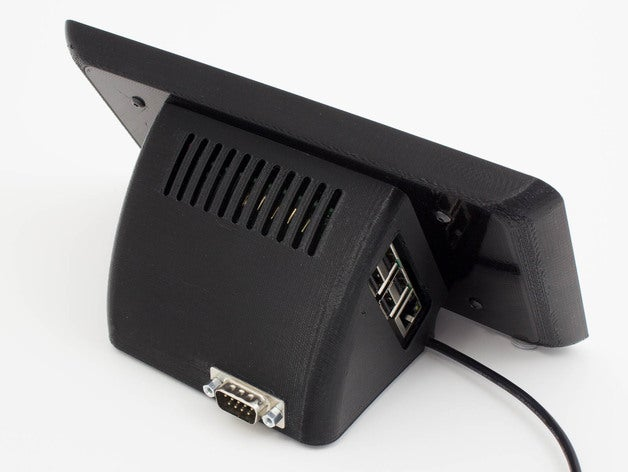
\includegraphics[height=2.5in]{figures/raspberrypicase7_preview_featured.jpg}
\caption[Carcasa de raspberryPi con Panel]{Carcasa de raspberryPi con Panel diseñado por James Clough\footnotemark}
\end{figure}

\section{Estableciendo un asistente inteligente para la gestión de la suite domótica}
\label{ch:Capitulo6.5}

El modelo actual del frontend y el backend han sido diseñados con buenas capas de abstracción con el fin de poder seguir creciendo tanto horizontal como verticalmente. El sistema actual por el cual la aplicación móvil es informado por el servidor del estado actual de las habitaciones y los dispositivos permitiría añadir una funcionalidad de notificaciones inteligentes, mediante las cuáles enviaría un aviso a la aplicación móvil cuando el servidor detectase ciertos eventos o patrones, parametrizables por el usuario. Así, cuando el servidor detectara un incremento lento pero gradual de la temperatura en una habitación durante el día, notificaría al dispositivo móvil dicho evento y sugeriría al usuario que decidiera si bajar las persianas o encender el aire acondicionado de dicha habitación.

\section{Desplegando informes de evolución histórica de medidas capturadas}
\label{ch:Capitulo6.6}

En la misma línea que la sección anterior, se puede añadir una funcionalidad adicional que a la hora de calcular los datos generales de cada habitación guarde un estado particular de dicha habitación en otra colección con el objetivo de establecer un historial de mediciones. De esta manera, se podría no sólo controlar la evolución de cada una de esas mediciones y detectar posibles anomalías mostrándole al usuario detalladas gráficas, por ejemplo, de temperatura y humedad para una habitación en particular, sino además utilizar dicha información como base para la detección de patrones por el asistente inteligente descrito anteriormente.

\section{Valoración de impacto ambiental}
\label{ch:Capitulo6.7}

Se ha determinado depositar todos los componentes dañados durante el proceso de estudio de hardware, y aquellos que en el futuro dejen de funcionar en los puntos limpios de recogida establecidos por la comunidad de Madrid más cercanos. El uso del material de impresión \verb|PLA| en las cubiertas de componentes como la Raspberry Pi no esta basado en petroleo y está considerado de bajo impacto medioambiental en su uso, sin embargo, no es un material reciclable como el caso del \verb|ABS| que es procesado para crear pellets con el fin de crear nuevos componentes plásticos, pero, al tratarse de un material fabricado en base a plantas como el maíz, es biodegradable en un rango de tiempo de unos meses si se aplica correctamente la técnica de compostaje. Por ello los restos de impresión, piezas no válidas o defectuosas en el proceso de creación serán depositadas en los cubos de basura orgánicos.